\documentclass[twoside,12pt]{article}

\usepackage{dsctemplate}
\usepackage[margin=1in]{geometry}
\usepackage{amsmath}
\usepackage{amssymb,amsthm}
\usepackage{fancyhdr}
\usepackage{nicefrac}
\usepackage{minted}
\usetikzlibrary{quotes,angles,positioning,arrows.meta}
\usetikzlibrary{calc}
\usepackage{enumitem}
\usepackage{fancyvrb}
\usepackage{dirtytalk}


\DefineVerbatimEnvironment{verbatim}{Verbatim}{xleftmargin=.5in}

% \renewcommand{\rmdefault}{phv} % Arial
% \renewcommand{\sfdefault}{phv} % Arial

% configuration
% ------------------------------------------------------------------------------

% control whether solutions are show or hidden
\showsolntrue

% page headers only on odd pages
\pagestyle{fancy}
\fancyhead{}
\fancyhead[RO]{PID or Name: \rule{3in}{.5pt}}
\renewcommand{\headrulewidth}{0pt}

% ------------------------------------------------------------------------------

\begin{document}

\thispagestyle{empty}

\begin{center}
    \noindent \textbf{\large{Data Overview: Cost of Living}} 
\end{center}


\noindent An area's cost of living describes how expensive it is to live in that area. In this exam, we'll work with the DataFrame \texttt{living\_cost}, which describes the typical cost of living for different types of families across all $3143$ counties in the 50 United States. The first few rows of \texttt{living\_cost} are shown below, but \texttt{living\_cost} has \textbf{many more rows} than shown.

\begin{center}
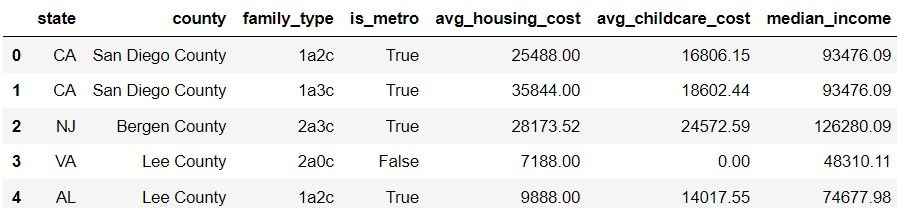
\includegraphics[width=\textwidth]{midterm_images/living_cost_preview.jpg}
\end{center}

\noindent Two counties in the same state will never have the same name, but as rows 4 and 5 above illustrate, there are some counties in different states with the same name, like Lee County.

\vspace{0.1in}

\noindent The \texttt{"family\_type"} column uses a code to describe the number of adults and children in a family. For example, a value of \texttt{"2a1c"} represents families with two adults and one child. There are ten unique values, as follows: \texttt{"1a0c"}, \texttt{"1a1c"}, \texttt{"1a2c"}, \texttt{"1a3c"}, \texttt{"1a4c"}, \texttt{"2a0c"}, \texttt{"2a1c"}, \texttt{"2a2c"}, \texttt{"2a3c"}, \texttt{"2a4c"}. We will assume that \textbf{all families fall into one of these ten categories}, and \textbf{all ten family structures are present in each US county}.

\vspace{.1in}

\noindent Each of the $31430$ rows of the DataFrame represents a unique combination of \texttt{"state"}, \texttt{"county"}, and \texttt{"family\_type"}. As a result, there will be more than one row with a \texttt{"state"} of \texttt{"CA"} and a \texttt{"county"} of  \texttt{"San Diego"}, corresponding to different values of \texttt{"family\_type"}. Similarly, there will be many rows such that \texttt{"family\_type"} is \texttt{"2a1c"}, all corresponding to different counties.  There is \textbf{only one row}, however, where \texttt{"state"} is \texttt{"CA"},  \texttt{"county"} is  \texttt{"San Diego"}, and  \texttt{"family\_type"} is \texttt{"1a2c"}

\vspace{.1in}

\noindent In addition to the \texttt{"state"}, \texttt{"county"}, and \texttt{"family\_type"} columns, \texttt{living\_cost} includes the following columns.

\begin{itemize}
    \item \texttt{"is\_metro" (bool)}: \texttt{True} if the county is part of a metropolitan (urban) area, \texttt{False} otherwise.  This value is the same for all rows of the DataFrame corresponding to the same county and state.
    \item \texttt{"avg\_housing\_cost" (int)}: The average yearly cost of housing, in dollars, for families of the given size in the given county and state.
    \item \texttt{"avg\_childcare\_cost" (int)}: The average yearly cost of childcare, in dollars, for families of the given size in the given county and state.
    \item \texttt{"median\_income" (int)}: The median annual income, in dollars, for families of the given size in the given county and state.

    
\end{itemize}


\vspace{.1in}

\noindent \textbf{Throughout the exam}, assume we have already run \texttt{import babypandas as bpd} and \texttt{import numpy as np}.




\end{document}
